
\chapter{IMAX3 Hardware}

\section{Chiplet and Vector Length}

\begin{figure}[htbp]
\center
\includegraphics[angle=270,origin=b,width=0.85\textwidth]{fig01.eps}
\caption{\label{fig:vl}Variation of Vector Length}
\end{figure}

\begin{figure}[htbp]
\center
\includegraphics[angle=270,origin=b,width=0.32\textwidth]{fig02.eps}
\includegraphics[angle=270,origin=b,width=0.32\textwidth]{fig03.eps}
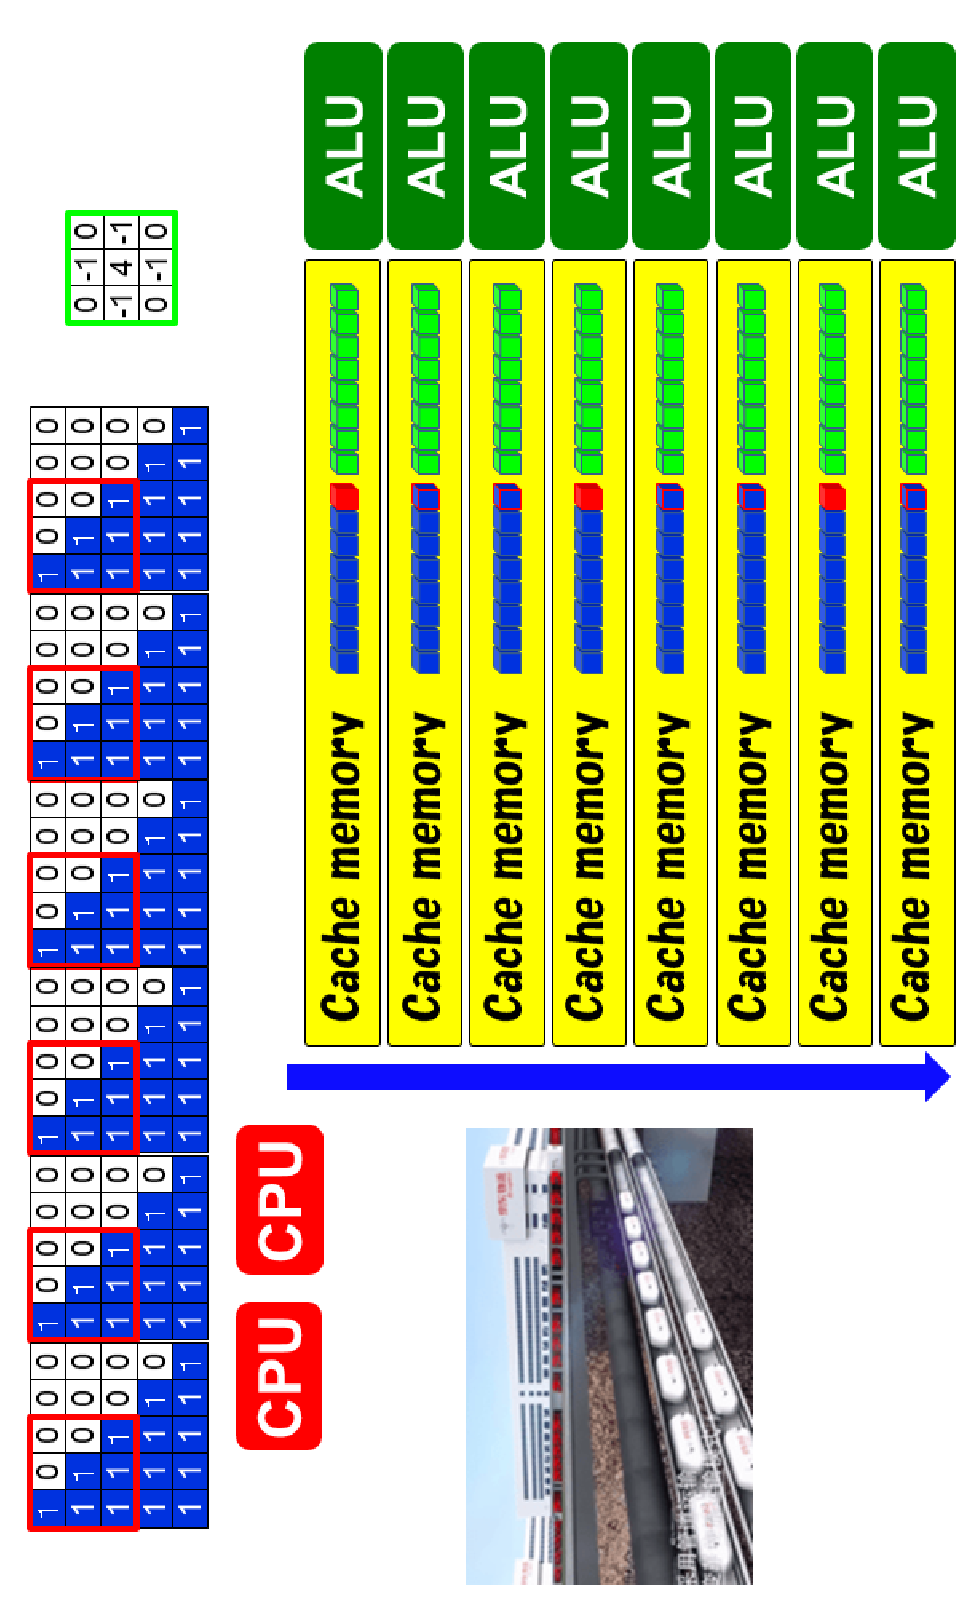
\includegraphics[angle=270,origin=b,width=0.32\textwidth]{fig04.eps}
\caption{\label{fig:comp}Multicore system, GPGPU and CGRA}
\end{figure}

Chiplets require sufficient vector length to minimize chip-to-chip data
transfer overhead. And IMAX3 is a chiplet-oriented architecture. Let's look
at the vector length in Fig.\ref{fig:vl}. A scalar processor has SIMD for
about 32 elements.  SIMD for 256 elements or more is called a vector. Vector
1 is connected to the cache memory.  Vector 2 is directly connected to the
main memory, and the vector length is about 2048.  The CGRA can have a
sandwich structure of ALU and 64KB of cache memories. The vector length is
now 16K.  By encapsulating irregular access patterns in cache memory, the
main memory can keep high speed with regular access patterns.

Figure\ref{fig:comp} illustrates typical execution models. Let's assume one
car is one CPU.  Blue data is the input image, and green data is the weight.
Every CPU tries to get the missing data in cache memory, even if it's the
same, and we cannot estimate when the data will arrive. GPGPU also has many
cores, but the cars are aligned and coalesced as much as possible before
they depart.  By merging the departure and arrival, we can reduce traffic
congestion.  However, if the destinations are scattered, GPGPU can do
nothing.  Whether coalescing is possible or not depends on the programming
skill. The right side is IMAX.  There are a few CPUs on top.  A lot of cache
memories do not go to get data and wait for the data provided by the CPU.
The CPU can send the green weight data at once.  We can reduce the amount of
data transmission and energy.

\section{Independent network for memory and execution}

\begin{figure}[htbp]
\center
\includegraphics[angle=270,origin=b,width=0.80\textwidth]{fig05.eps}
\caption{\label{fig:mesh}Execution network and Memory network}
\end{figure}

\begin{figure}[htbp]
\center
\includegraphics[angle=270,origin=b,width=0.80\textwidth]{fig06.eps}
\caption{\label{fig:ring}IMAX2 multichip structure}
\end{figure}

\begin{figure}[htbp]
\center
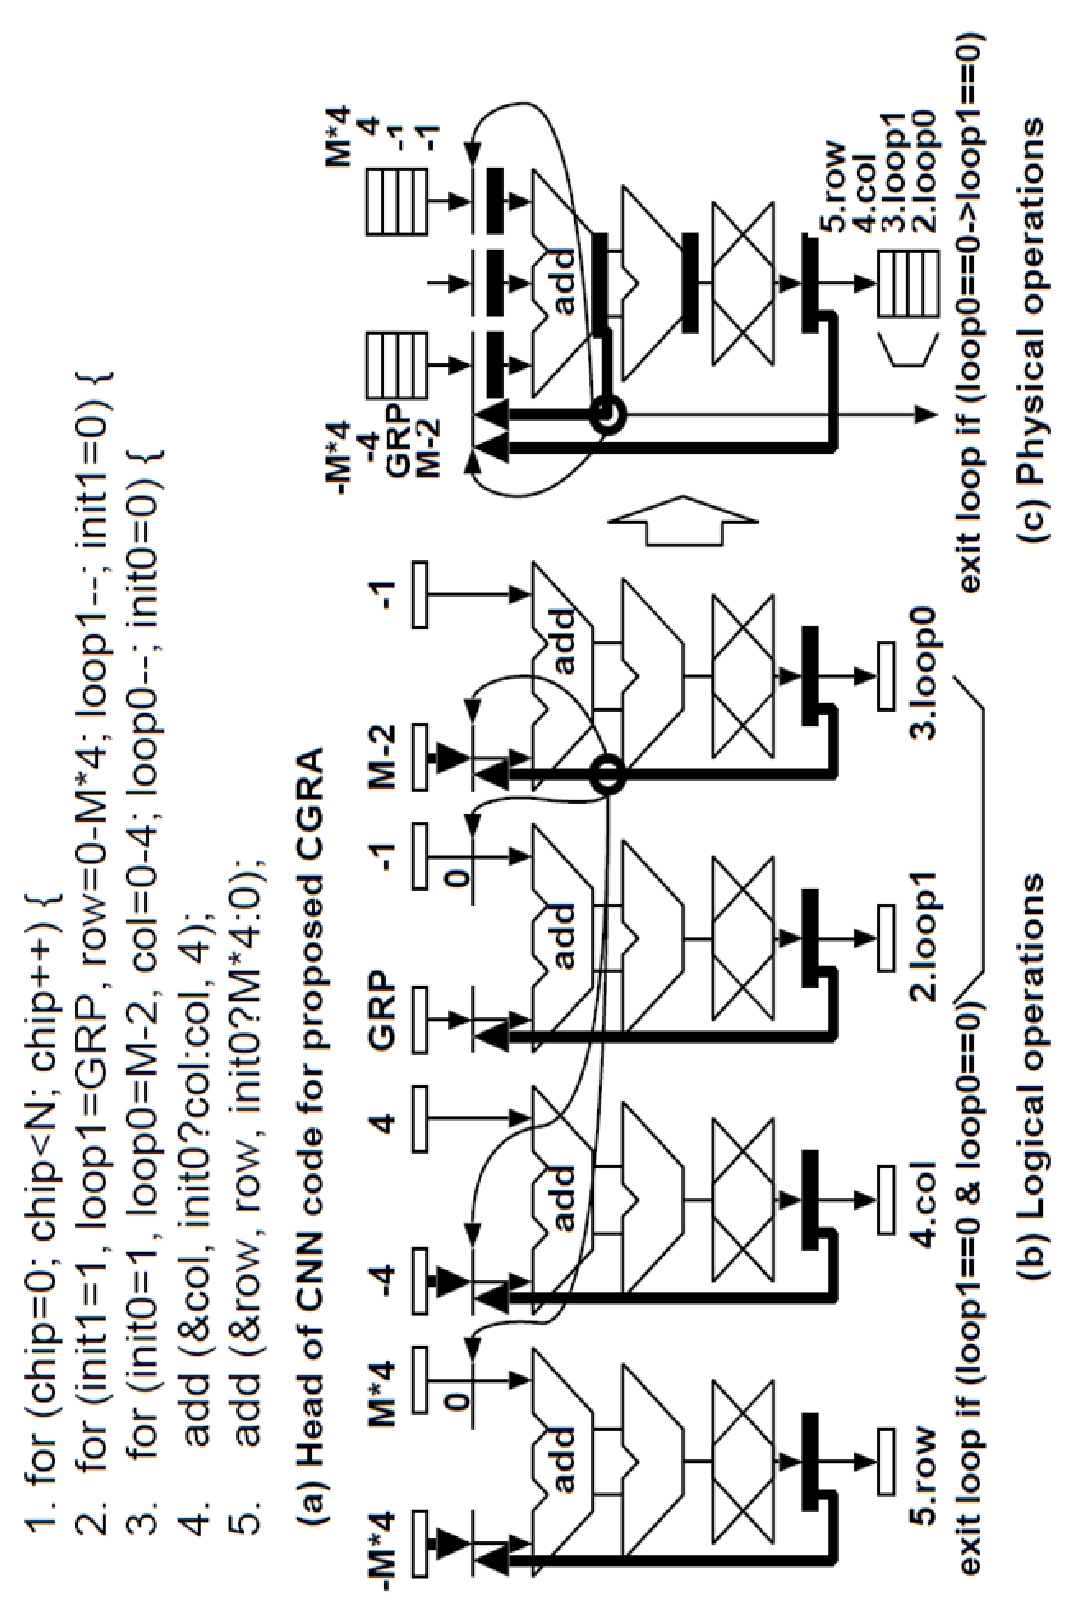
\includegraphics[angle=270,origin=b,width=0.80\textwidth]{fig30.eps}
\caption{\label{fig:loopctrl}Burst execution of triple loops}
\end{figure}

\begin{figure}[htbp]
\center
\includegraphics[angle=270,origin=b,width=0.80\textwidth]{fig33.eps}
\caption{\label{fig:multilane}IMAX3 multilane structure}
\end{figure}

As shown in Fig.\ref{fig:mesh}, there are two types of networks in
IMAX2. The latency is reduced by grouping eight units and connecting them in
parallel to the memory interface. For computation, 64 units are connected in
a ring within each chip, and the combination of computation and local memory
can be changed like a combination lock.  A ring structure is helpful for
stencil computations. By sliding the mapped operations, the pair of ALU and
cache memory can be adjusted. Much of the data in cache memory can be
reused.  To reduce the overhead, the triple loop can be mapped on IMAX as
shown in Fig.\ref{fig:ring}. The outermost loop is mapped on multiple chips,
and the inner double loop is mapped on each chip. Fig.\ref{fig:loopctrl}
illustrates how four logical units (one physical unit) manage the triple
loops. IMAX3 has multiple memory ports and multiple IMAX2 lanes, as shown
in Fig.\ref{fig:multilane}.

\section{Multilevel pipelining}

\begin{figure}[htbp]
\center
\includegraphics[angle=270,origin=b,width=0.80\textwidth]{fig07.eps}
\caption{\label{fig:micro}Micro pipelining}
\end{figure}

\begin{figure}[htbp]
\center
\includegraphics[angle=270,origin=b,width=0.80\textwidth]{fig08.eps}
\caption{\label{fig:medium}Medium pipelining}
\end{figure}

\begin{figure}[htbp]
\center
\includegraphics[angle=270,origin=b,width=0.80\textwidth]{fig09.eps}
\caption{\label{fig:macro}Macro pipelining}
\end{figure}

\begin{figure}[htbp]
\center
\includegraphics[angle=270,origin=b,width=0.80\textwidth]{fig10.eps}
\caption{\label{fig:all}Multilevel pipelining}
\end{figure}

\begin{figure}[htbp]
\center
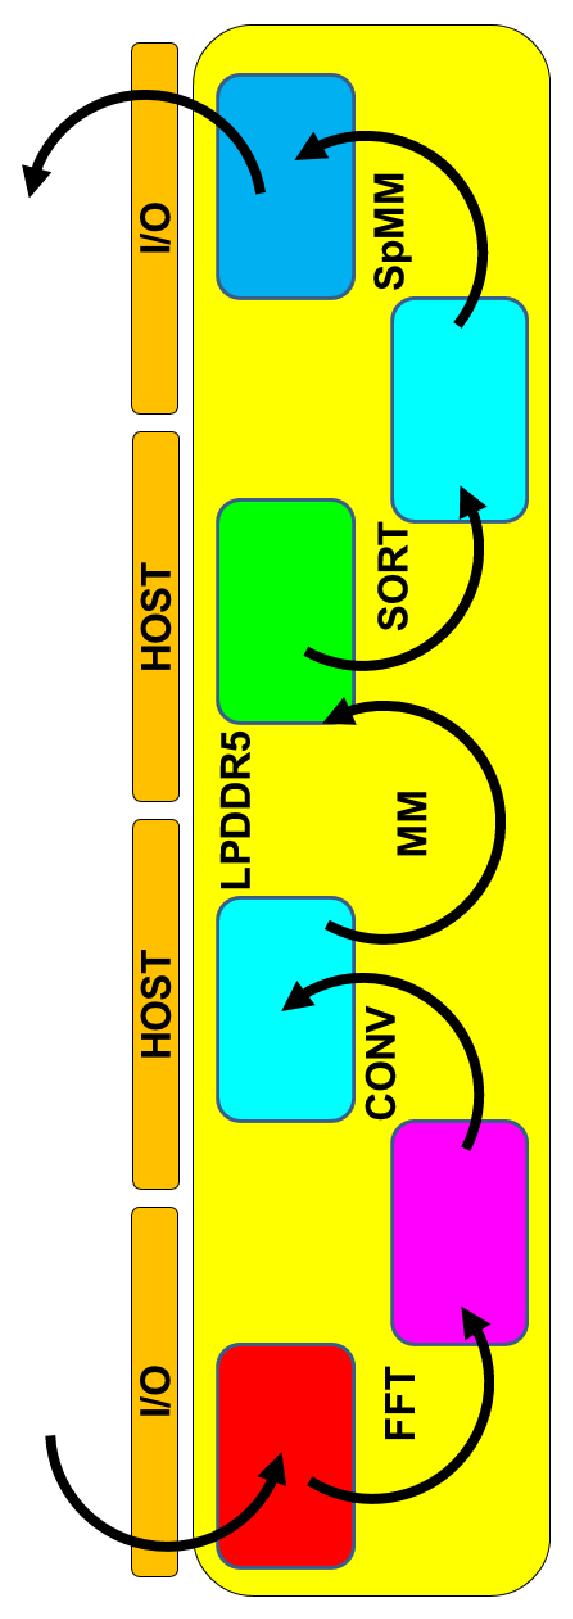
\includegraphics[angle=270,origin=b,width=0.80\textwidth]{fig11.eps}
\caption{\label{fig:map}Mapping of application kernels}
\end{figure}

Figure\ref{fig:micro} illustrates the multiple lanes of IMAX2 connected to
LPDDR5 memory, and the first level (micro) pipelining in each lane.  The micro
pipelining is the basic mode of CGRAs.  Each lane may have multiple IMAX2
chips.  This mode can follow the traditional and sequential program, and can
reduce the compilation time.  Figure\ref{fig:medium} illustrates the
multiple lanes of IMAX2 and the second level (medium) pipelining in each
lane.  The medium pipelining is provided by the double buffering in cache
memory blocks in each lane, and can follow the multiple stages in sorting,
hash function, and FFT. Figure\ref{fig:macro} illustrates the macro
pipelining of IMAX3.  The multiple lanes are concatenated as a pipeline
through LPDDR5.  Each lane may have micro and medium pipelining.
Figure\ref{fig:all} shows the final goal of IMAX3. Each lane has multiple
IMAX2 chips.  Many lanes and CPUs are employed, and many kinds of kernels
are mapped simultaneously as shown in Fig.\ref{fig:map}.

\begin{figure}[htbp]
\center
\includegraphics[angle=270,origin=b,width=0.80\textwidth]{fig12.eps}
\caption{\label{fig:chip}Area estimation}
\end{figure}

\clearpage

\section{Prototype}

\begin{figure}[htbp]
\center
\includegraphics[angle=270,origin=b,width=0.80\textwidth]{fig13.eps}
\caption{\label{fig:proto}Prototype of IMAX3}
\end{figure}

\begin{figure}[htbp]
\center
\includegraphics[angle=270,origin=b,width=0.80\textwidth]{fig14.eps}
\caption{\label{fig:evmodel}Evaluation models}
\end{figure}

As shown in Fig.\ref{fig:chip}, 75\% area of IMAX3 is memory blocks. If each
port of the LPDDR5 has four modules of 64-unit IMAX, 10240 operations can be
mapped. If 30 ports are available, 307200 operations can be mapped. If we
can fabricate with 8nm technology, 120 modules of IMAX will occupy the 144mm
square.  Figure\ref{fig:proto} is the ongoing project to scale up the IMAX2
to IMAX3. VPK180 has two sets of IMAX2 and can connect eight IMAX2 through
the NoC. Figure \ref{fig:evmodel} is a performance evaluation model using a
prototype. Eight units will be implemented: IMAX2\#0.0, IMAX2\#1.0, ...,
IMAX2\#7.0. Each IMAX2 corresponds to a configuration of NLANE=8 and NCHIP=1
in the IMAX2 application program. On the other hand, it is also possible to
run the IMAX2 application program by writing NLANE=8 and NCHIP=6. This
method corresponds to a configuration with multiple IMAX2 lanes in a cascade
configuration. However, since only the first IMAX2\#*.0 is implemented, the
execution result of subsequent IMAXs connected in cascade will be 0, and the
overhead associated with cascade connection will not be measured. The
execution speed is just a ideal value.
